\documentclass[12pt,letterpaper]{article}
\usepackage[utf8]{inputenc}
\usepackage{amsmath}
\usepackage{amsfonts}
\usepackage{amssymb}
\usepackage{graphicx}
\usepackage{fourier}
\usepackage{fullpage}
\usepackage{caption}
\author{Christopher C. Lamb, Gregory L. Heileman \\
{\small \{cclamb, heileman\}@unm.edu}}
\title{UNM Informatics OVPR Equipment Funding Request}
\date{}
\begin{document}

\maketitle

%\abstract{
%{\sl\noindent The Informatics Group affiliated with the Electrical and Computer Engineering Department has a small cloud laboratory that we have been building for the past three years. We have spent initial funding, and need to replace some of the older systems as well as acquire additional systems to both effectively teach students affiliated with the laboratory and to compete for research grants. This will allow us to collaborate more effectively in national security and network research, better compete for funding, and help our students prepare for the future technology market.}
%}

\section{Significance of Current Need}
Students need to be prepared to support computing needs in distributed utility-style computing environments. This Cloud Computing paradigm is pervasive, affecting engineers throughout the computer engineering and science landscape. Engineers today deploy systems to cloud computing environments, manage availabilty through cloud computing toolsets, and provide enhanced application experience via cloud computing infrastructure. Likewise, network and systems engineers are required to understand how to implement large-scale cloud environments in Cloud Service Provider (CSP) environments like those managed by large scale providers including Amazon\footnote{http://aws.amazon.com, a principal cloud service provider.} and Rackspace\footnote{http://www.rackspace.com, a company that provides various infrastructure-as-a-service offerings.}. Via this grant, we propose to provide an environment in which students can gain experience with cutting edge computer technologies they need to understand in today's market, as well as enhance our abilty to support graduate students via external grant acquisition.

\begin{figure}[!t]
\centering
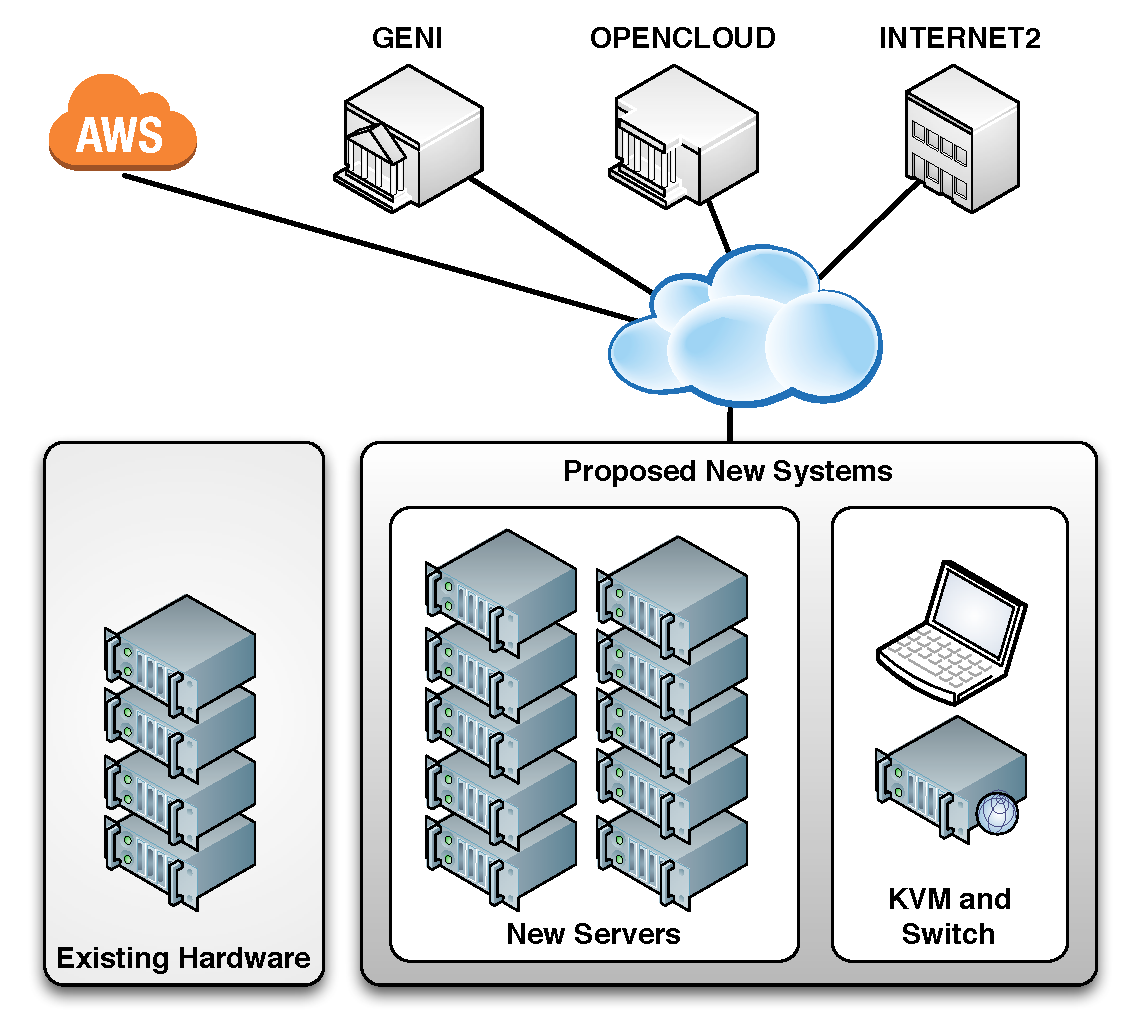
\includegraphics[width=0.9\textwidth]{images/system.pdf}
\caption{The overall system after new system acquisition showing collaboration potential.}
\label{fig:conops}
\end{figure}

\paragraph{Research Support} We are currently teaching students how to provide cloud services via outdated infrastructure, and much of our networking research is only supportable via simulation. The proposed hardware will fit in our current computer room, using previously acquired server rackspace. This will enable our students to use OpenFlow for software defined networking (SDN) and network functions virtualization (NFV) research, an area that is beginning to transform how we communicate via computer networks today by virtualizing networks just as we have virtualized server systems. Cloud computing was a \$130 billion market in 2013\footnote{http://www.gartner.com/newsroom/id/2352816}, and our students need to be prepared to engineer the future this this new world.

\paragraph{Enhancing Grant Competitiveness} During the last SBIR/STTR round, much of the computational engineering research focused on cloud computing and cyber-security. In order to compete effectively, organizations need access to a wide variety of cloud computing resources, ranging from external CSP access to internal configurable cloud computing infrastructure. We currently are able to run a very limited cloud computing environment using OpenStack\footnote{http://www.openstack.org} to support our cloud needs and OpenDaylight\footnote{http://www.opendaylight.com} for SDN. Not only is this insufficient for current needs, we are unable to supply access to external collaborators or other UNM students and professors. We furthermore are unable to join any of the large SDN network testbeds\footnote{http://www.opencloud.us, http://www.geni.net} as we lack the appropriate hardware to effectively collaborate. This grant will provide the needed resources for us to collaborate with the external research community and share our environment with other collaborators.

\paragraph{Student Support} Enhancing our grant competitiveness and providing an environment capable of hosting research into future computation techniques and infrastructure management provides our students with educational opportunities they currently do not have. Furthermore, our enhanced ability to secure additional grant funding provides a way for us to financially support more graduate students. More supported graduate students with more marketable skills translates into a stronger Engineering and UNM community moving into the future.

\begin{figure}[!t]
\centering
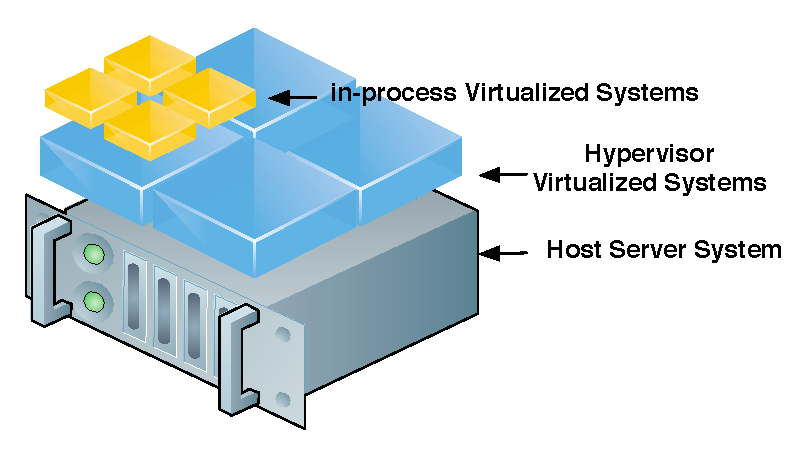
\includegraphics[width=0.9\textwidth]{images/virtualization.pdf}
\caption{Our virtualization strategy;  multiple in-process VMs hosted on hypervisor-based VMs.}
\label{fig:virtual}
\end{figure}

\subsection{Technical Proposal}
Figure~\ref{fig:conops} shows the system after the inclusion of the new servers and infrastructural hardware. We currently have four existing systems --- three older Dell systems (circa 2010) and a new HP Proliant system. The HP system will be integrated into our primary processing fabric, working and actively sharing load with computational systems. The older systems will transition to running low priority loads and SDN controller software (e.g. OpenDaylight). 

The proposed systems will become active computational nodes upon which we will run some number virtual machines (VMs) depending on load and VM requirements. These VMs will then host in-process virtualization images that host specific services as shown in Figure~\ref{fig:virtual}. We will reserve some arbitrary number of systems for Mininet\footnote{http://mininet.org} simulations as needed, and dynamically manage the availability of all systems via the SDN switch. We will also dedicate some number of systems to collaborative work with various network testbeds. At any given time, we will likely have two systems used for network simulations, two systems used for collaborative work, and seven systems reserved for other cloud provisioning experiments by Informatics personnel, students, or other internal collaborators.

We expect to tie our systems to the wider UNM authentication and authorization system to ease management and make resources more freely available.

\newpage
\section{Budget Summary}

\begin{table}
\center
\begin{tabular}{l*{6}{c}r}
Equipment	& Quantity & Cost/unit & Total cost \\ 

\hline\hline

HP 3500yl 48 port SDN switch {\small (J9311A)} & 1 & \$3,800.00 & \$3,800.00 \\ 
Dell TrippLite 8-Port 1U Console/KVM {\small (B020-U08-19-K)} & 1 & \$1,449.99 & \$1,449.99 \\
Dell PowerEdge R630 {\small (2 Xeon\textsuperscript{\textregistered} E5-2603 v3, 16GB RAM)} & 10 & \$2,686.90 & \$26,689.00 \\
Misc Cables &  &  & \$500.00 \\

\hline

Total &  &  & \$32,438.99  

\end{tabular}
\caption{The overall grant cost breakdown.}
\label{table:budget}
\end{table}

The equipment proposed includes a SDN switch with ports for expansion, a rackmountable console and KVM, 10 servers, and funding for miscellaneous cables and connectors. Today, Hewlett Packard has the most reasonably priced SDN switches, supporting the 1.3 version of the OpenFlow standard\footnote{https://www.opennetworking.org/images/stories/downloads/sdn-resources/onf-specifications/openflow/openflow-spec-v1.3.0.pdf}. We furthermore need a rackmountable console to allow us to manage the server systems, of which we intend to install ten. We have also allocated funding for various cables as needed. The overall budget allocation and equipment we intend to purchase is detailed in Table~\ref{table:budget}.


\newpage
\section{Principal Investigators}
Dr. Christopher Lamb and Dr. Greg Heileman currently run the Informatics Laboratory in the Electrical \& Computer Engineering department at the University of New Mexico. At any given time, they have on the order of 20 students involved in research, development, and various other engineering work at the undergraduate, master's, and PhD level.

{\bf Christopher C. Lamb} (cclamb@unm.edu) currently serves as a cyber-security Research Scientist with Sandia National Laboratories (SNL) and as a Research Assistant Professor affiliated with the Electrical and Computer Engineering department at the University of New Mexico (UNM). He currently participates in a wide range of research roles at SNL, ranging from analyzing moving target defense controls to designing neural algorithms for custom hardware implementation. At UNM, he leads students in research projects focusing on the security of software defined networking and cloud systems as well as academic analytic visualization and secure drone video capture and analysis. He also has extensive experience designing and developing mission-critical distributed systems for a wide range of government departments and agencies. Prior to joining SNL, Dr. Lamb served in executive roles and as a principal consultant for a variety of technology companies in the southwest. Dr. Lamb has a B.S. in Mechanical Engineering from New Mexico State University, an M.S. in Computer Science from the University of New Mexico, as well as a Ph.D. in Computer Engineering with a focus on Computational Intelligence from the University of New Mexico. He is an Open Group Architecture Framework (TOGAF) 9 Certified Enterprise Architect and a Certified Information Systems Security Professional (CISSP) through the International Information Systems Security Certification Consortium.

{\bf Gregory L. Heileman} (heileman@unm.edu) serves as the Associate Provost for Curriculum at the University of New Mexico (UNM), a position he has held since 2011.  He received the BA degree from Wake Forest University in 1982, the MS degree in Biomedical Engineering and Mathematics from the University of North Carolina-Chapel Hill in 1986, and the Ph.D. degree in Computer Engineering from the University of Central Florida in 1989.  In 1990 he joined the Department of Electrical and Computer Engineering (ECE) at UNM, where he is currently a Professor. From 2005-2011 he served as ECE associate chair (director of undergraduate programs), and led the department through two ABET accreditation visits.  In 2011 he became an ABET program evaluator. 

\end{document}